\documentclass[prl, reprint, twocolumn]{revtex4-1}
\usepackage[utf8]{inputenc}
\usepackage{blindtext}
\usepackage{graphicx}
\usepackage{braket}
\graphicspath{{figures/}}


%\renewcommand{\blindtext}{ }
\begin{document}
	\title{Weakly supervised learning of many-body quantum phases \\ via asymptotic phase classification}
	\date{\today}
	\author{Benjamin Claßen}
	\author{Titus Franz}
	\author{Matthias Weidemüller}
	\affiliation{Physikalisches Institut Heidelberg}
	\begin{abstract}
		
		Main messages:
		\begin{itemize}
			\item Application of the “Confusing Neural Network” method to a Heisenberg model
			\item New method for applying machine learning to a general class of many-body Hamiltonians
			\item Weakly supervised learning of many-body quantum phases via asymptotic phase classification
		\end{itemize}
		
	\end{abstract}
	\maketitle
	
	\section{Introduction}

	The recent advances in applications of Machine learning to a very diverse set of problems have quickly raised the question whether the study of many-body systems can also be advanced by employing methods of the very well equipped, general and accessible toolbox provided by the machine learning community.
	If a model can find structure within millions of megapixel images \cite{Needed}, can it maybe also cope with the vast Hilbert space of a many body system?
	
	In the short history of applying machine learning to many body systems, several different research directions have been pursued. It is possible to parameterize the wave function of a quantum spin system such that it can be mapped to a restricted Boltzmann machine, which translates variational principles to training a neural network\cite{Carleo2016a}. Using the same model, it is also possible to accelerate Monte-Carlo simulations \cite{Huang2017}. This paper will focus mainly on observable-based learning of the phase diagram of many body systems introduced by \cite{Carrasquilla2017}. In this approach, a neural network is used as classifier and trained on discriminating 2 phases of matter. \cite{Nieuwenburg2017} then generalized this approach to map out phase diagrams in an unsupervised fashion by introducing the confusion scheme which will be outlined in the next section.
	
	We will now introduce the XXZ-Heisenberg model and apply the confusion scheme to it. We then introduce a novel method for the prediction of phase diagrams and apply it to the same model. Finally, both methods will be compared with regards to required parameters, prediction quality and runtime performance.
	
	
	
	\subsection{The XXZ Heisenberg model}
	\begin{equation}
	H = J\sum_i^L\left(\sigma^x_i\sigma^x_{i+1}+\sigma^y_i\sigma^y_{i+1}+\Delta\sigma^z_i\sigma^z_{i+1}\right) - h_x\sum_i^L\sigma^x_i
	\label{eq:xxz}
	\end{equation}
	
	
	\section{The unsupervised confusion scheme}
	Building on the observable-based detection of phase transition as introduced by Carrasquilla et al \cite{Carrasquilla2017}, an unsupervised scheme to scan phase diagrams was introduced by Nieuwenburg et al. \cite{Nieuwenburg2017}.
	While neural networks can natively be used in an unsupervised fashion by using autoencoders for example - these have even been used on many-body problems \cite{Wetzel2017} - the confusion scheme is completely agnostic with regard to the machine learning model used. It is based on the idea that a classifier will perform best if the training data is labeled correctly. By proposing different critical points, labeling the data accordingly and by training a machine learning model on each of these propositions, the classifier is expected to perform best on the proposed critical point closest to the correct critical point.
	
	This approach can be generalized to scan a phase diagram by a sliding window approach\cite{Broecker2017}. Two points $\lambda_1$, $\lambda_2$ within the phase diagram are selected and are proposed to lie within two different phases. A classifier is trained on these two points and the response $p$ when predicting the class of the test data between the 2 training points is recorded. We quantify the probability $P$ that the two points $\lambda_1$ and $\lambda_2$ lie in 2 different phases, i.e. there is a phase transition between the two points as
	
	\begin{equation}
	P = 2\frac{\int_{\lambda_1}^{\lambda_2} d\lambda |p(\lambda) - 0.5|}{\lambda_2-\lambda_1}
	\label{eq:P}
	\end{equation}
	
	By scanning the full phase diagram, training a classifier for every point of the discretized space, $P$ displays phase outlines.
	
	There are 2 main parameters to choose for this method: the window width $|\lambda_2-\lambda_1|$ and for phase diagrams of more than one dimension the scan direction has to be considered: If the line segment $\overline{\lambda_1\lambda_2}$ is parallel to a phase boundary, this phase boundary will not be detected.
	Therefore, it was decided to scan once along each axis.
	
	
	
	\subsection{Application of the unsupervised confusion scheme \\ to the XXZ model}
	We simulate the XXZ model's ground state using Matrix Product states\cite{Schollwoeck2011} using the two-site variational ground state search as implemented in the OpenMPS library\cite{Jaschke2018, Wall2012}. The Hamiltonian \ref{eq:xxz} is formulated as Matrix Product Operator for a grid of ($h_x$, $\Delta$) values and the corresponding correlation matrix $\braket{\sigma^i_z\sigma^j_z}$ is recorded.
	
	The machine learning model that is used as classifier is a feed-forward, fully connected neural network with just one hidden layer of 100 neurons. Neural networks with more degrees of freedom did not improve the results. The classifier was not trained directly on the simulated correlation matrices, but on the discrete correlation functions $f(r) = \braket{\sigma^i_z\sigma^{i+r}_z}$.
	
	\begin{figure}[h]
		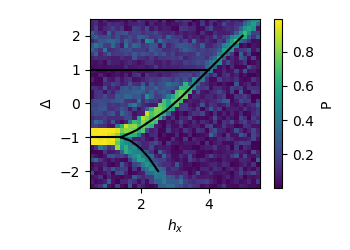
\includegraphics[width=\columnwidth]{3_5_ConfusionPhaseDiagram2D_1_20181214}
		\caption{Application of the confusion scheme to the XXZ model. The scan direction was parallel to the $\Delta$ axis and the window width was set to 0.5. The black line overlay corresponds found using mean field theory\cite{Dmitriev2002}. $P$ corresponds to the probability defined in \ref{eq:P}}
		\label{fig:confusion}
	\end{figure}
	
	The results of the confusion scheme are presented in \ref{fig:confusion}. We only present the scan parallel to the $\Delta$ axis as the scan parallel to the $h_x$  axis could not reveal any structure parallel to that axis. The two phases for $\Delta = 0$ and high $\Delta$ - values are separated by a crossover. Since the window width is only 0.5, the classifier is not able to reliably discriminate the two phases. But even when increasing the window width to 2, P did not increase along the line $\Delta=1$.
	
	\section{Weakly supervised learning \\ via asymptotic limits}
	The sliding window approach of the confusion scheme only considers a small local subset of the training data within the phase diagram for each of the trained classifiers.
	Since a classifier generally performs better with additional training points - given that the new points are labeled correctly and the model is not yet saturated with the existing training data \cite{}- a more global approach could provide better results.
	
	We therefore introduce a new method for automatic phase detection. We assume that the asymptotic behavior of the system is known and propose an initial guess of the phases. In the case of the XXZ model, for example, we assume four distinct phases for ($h_x=0$, $\Delta=0$), ($h_x=0$, $\Delta\rightarrow\infty$), ($h_x=0$, $\Delta\rightarrow -\infty$) and ($h_x=0$, $\Delta\rightarrow\infty$). We now train a single classifier for the entire phase diagram. We employ a very similar model and as in the previous approach, the only difference being that the output layer contains four neurons, each one trained to respond to the four phases proposed by asymptotic considerations.
	
	As for the training data, we still use the same correlation functions, but we select four subsets of the data in proximity of the four proposed phases and apply a different label to each subset. We the interpret the neuron response when inferring on the remaining correlation functions as phase diagram. 
	
	
	
	\subsection{Application of the asymptotically labeled scheme \\ to the XXZ model}
	\begin{figure}[h]
		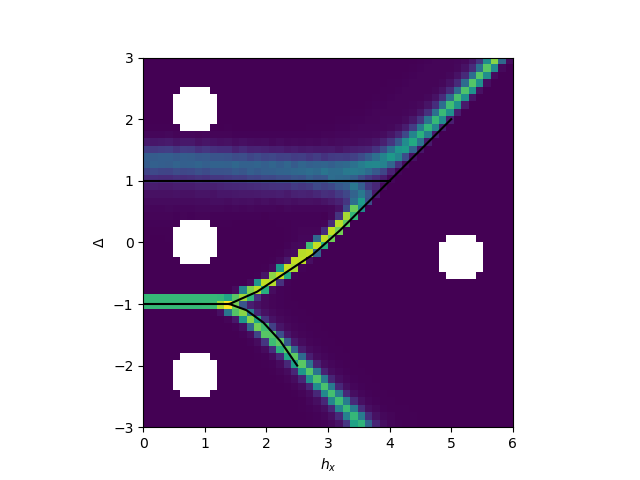
\includegraphics[width=\columnwidth]{3_6_Weak4PhaseDetection2DEdges_30_20190109}
		
		\caption{Phase diagram as obtained by the asymptotically labeled scheme. Color indicates the confidence of detecting a phase transition $P_a$, as defined in equation \ref{eq:Pa}. The white patches indicate the location of the training data. The black overlay is the phase diagram of the XXZ model as presented by \cite{Dmitriev2002}.}
		\label{fig:asymptotic:base}
	\end{figure}
	\begin{figure}[h]
		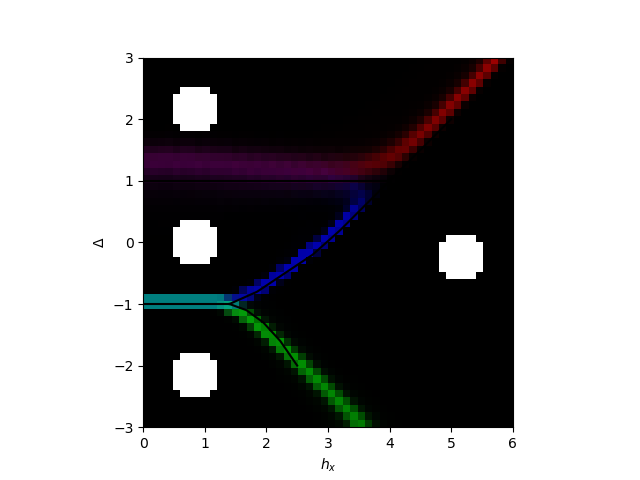
\includegraphics[width=\columnwidth]{3_6_Weak4PhaseDetection2DEdges_20_20190109}
		\label{fig:asymptotic:base1}
		\caption{Gradient over output of four neurons, interpreted as rgb color (first neuron red, second neuron green, third neuron blue, 4th neuron 1-rgb)}
	\end{figure}
	
	\begin{figure}[h]
		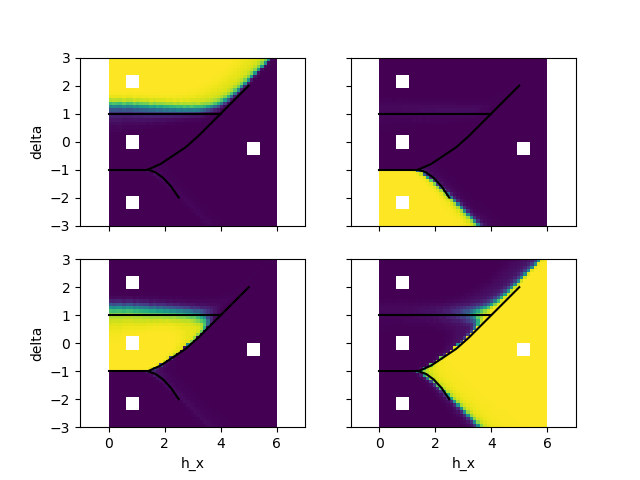
\includegraphics[width=\columnwidth]{3_6_Weak4PhaseDetection2D_10_20190109}
		\label{fig:asymptotic:base2}
		\caption{four neuron outputs as four plots, as in thesis. Most direct visualization, but takes up a lot of space}
	\end{figure}
	\begin{figure}[h]
		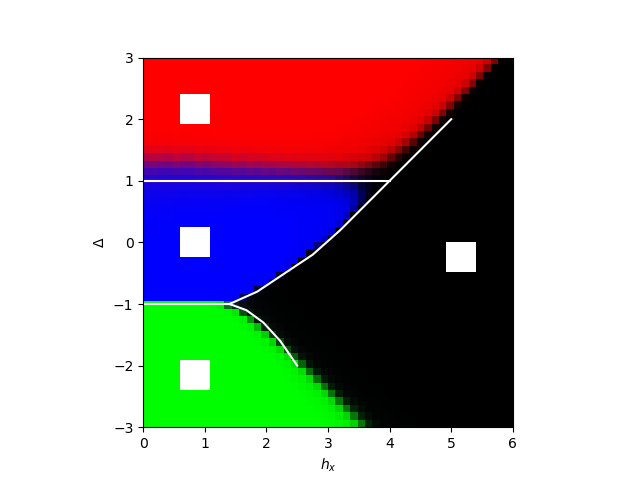
\includegraphics[width=\columnwidth]{3_6_Weak4PhaseDetection2DRGB_40_20190109}
		\label{fig:asymptotic:base3}
		\caption{neuron output interpreted as rgb color  (first neuron red, second neuron green, third neuron blue, 4th neuron 1-rgb)}
	\end{figure}
	The same dataset of MPS-simulated correlation functions of the XXZ model as used for the confusion scheme is also employed for the newly introduced scheme. Four patches of the phase diagram are labeled as phase guess \footnote{These appear as white patches in figure \ref{fig:asymptotic:base}} and the model is trained on discriminating these four training patches. The subset of the dataset not belonging to the training data is used as test data.
	
	We record the neuron response of the four output neurons for every test data point. To visualize the phase boundaries in a single diagram, we calculate the average gradient of the neuron responses $R$ according to
	
	\begin{equation}
		P_a = \frac{1}{4} \sum_{i}^4 \sqrt{(\partial_{h_x} R_i)^2 + (\partial_{\Delta} R_i)^2}
		\label{eq:Pa}
	\end{equation}
	
	and interpret $P_a$ as the model's confidence in detecting a phase transition.
	
	
	The resulting phase diagram is given in figure \ref{fig:asymptotic:base}. The phase diagram of the XXZ model as described in \cite{Dmitriev2002} is recovered. Even the crossover at $\Delta=1$ is detected, which was missed when applying the confusion scheme to this model (compare figure \ref{fig:confusion}). The fact that a crossover is observed is hinted by the much broader boundary in the predicted phase diagram, indicating that there is a larger region where our phase classifier cannot discriminate the phases with high confidence.  Overall, the resulting phase diagram is much less noisy when compared to the one obtained by the confusion method and no window width or scan direction needs to be chosen.
	
	Training the neural network of the asymptotic method needed for the full phase diagram took a similar amount of time as training the neural network of the confusion method needed for a single point within the phase diagram. For this problem, the asymptotic method therefore was 2-3 orders of magnitude faster than the confusion method.
 	
	\subsection{Robustness of the predicted phase diagram}
	While the asymptotic method does not depend on the hyperparameters window size and scan direction, the question remains whether the result is independent of the initial phase guess. We are especially interested in the following 2 considerations:
	\begin{enumerate}
		\item Will the phase boundaries be robust against a different initial phase guess?
		\item Is it possible to detect an erroneous phase guess i.e. either 2 proposed phases lie within the same phase or an existing phase is missing in the initial guess.
	\end{enumerate}

	\begin{figure}[h]
		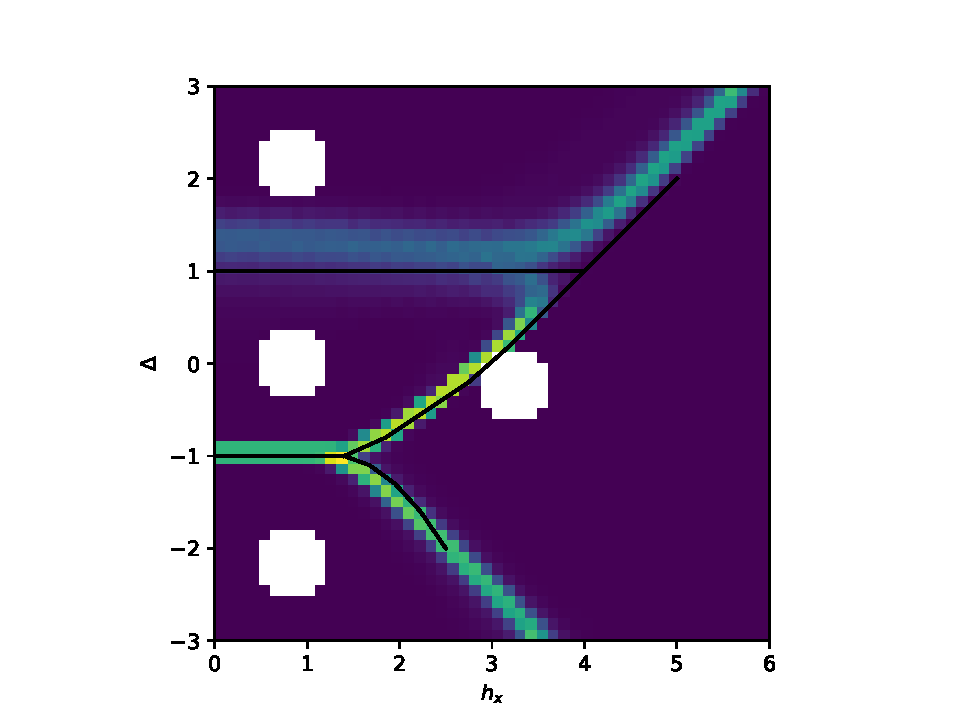
\includegraphics[width=\columnwidth]{3_6_Weak4PhaseDetection2DEdges_330_20190119}
		
		\caption{Robustness of the predicted phase diagram for an initial guess with training data close to a phase transition. Colors, patches and overlay as in figure \ref{fig:asymptotic:base}.}
		\label{fig:asymptotic:transition}
	\end{figure}

	\begin{figure}[h]
	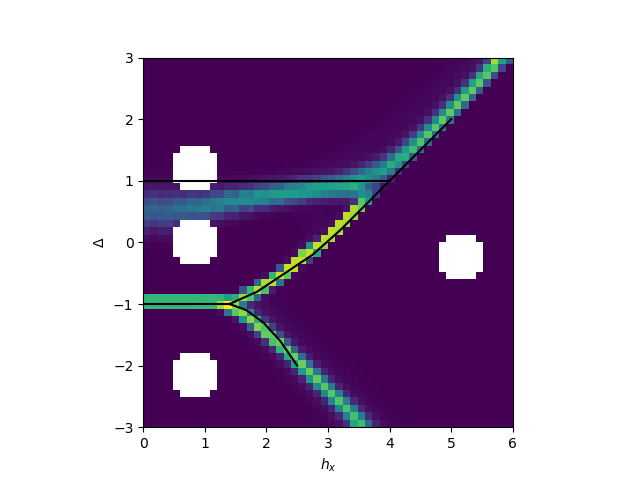
\includegraphics[width=\columnwidth]{3_6_Weak4PhaseDetection2DEdges_34_20190119}
	
	\caption{Robustness of the predicted phase diagram for an initial guess with a different training patch selection at the crossover between $\Delta=0$ and high $\Delta$ values. Colors, patches and overlay as in figure \ref{fig:asymptotic:base}.}
	\label{fig:asymptotic:crossover}
	\end{figure}

	To investigate the robustness of the predicted phase diagram, the selected training patches of figure \ref{fig:asymptotic:base} are moved closer to phase boundaries. Figure \ref{fig:asymptotic:transition} exemplifies this for the phase transition between low and high values of $h_x$ (along $\Delta=0$). The training patch can be brought arbitrarily close to the phase transition without any significant effect on the prediction. This has also been tested for all other phase transitions, but it does not apply to the crossover between low and high $\Delta$ values. As the corresponding patches are moved, the classifier can always discriminate between the two phases, but the exact location of the decision boundary between the two classes depends on the observed correlation functions during training. The phase classifier interpolates between the two different phases adjacent to the crossover. This behavior is presented in figure \ref{fig:asymptotic:crossover}. For a phase transition, the decision function of our classifier is invariant against variations in the training data. The classifier is able to extract the relevant features of each phase from training data in close proximity to or far away from the phase transition since there is a very defined step in the order parameter at the phase transition. If there are only smooth changes in the behavior of the system between two phases, the classifier will set an almost arbitrary threshold in between these phases. This still results in a training error of zero and full separation of the phases, but not in a robust phase boundary.
	

	\begin{figure}[h]
		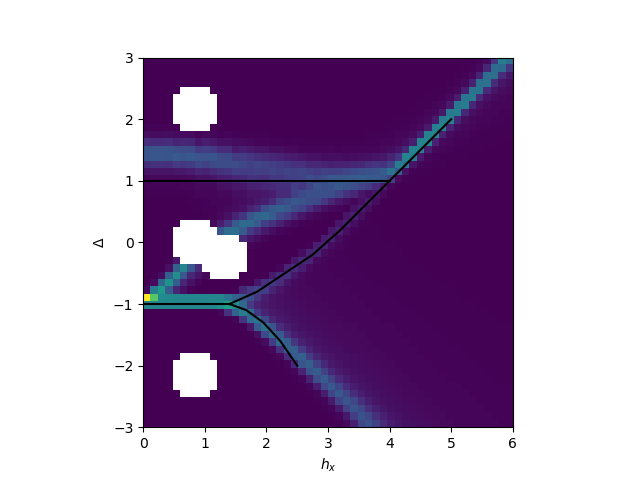
\includegraphics[width=\columnwidth]{3_6_Weak4PhaseDetection2DEdges_334_20190119}
		
		\caption{Robustness of the predicted phase diagram against an erroneous selection of training data: Two training patches within the same phase are labeled to be 2 different classes while the $h_x \rightarrow \infty$ phase is completely missing as class. Colors, patches and overlay as in figure \ref{fig:asymptotic:base}.}
		\label{fig:asymptotic:wrongguess}
	\end{figure}
	\begin{figure}[h]
		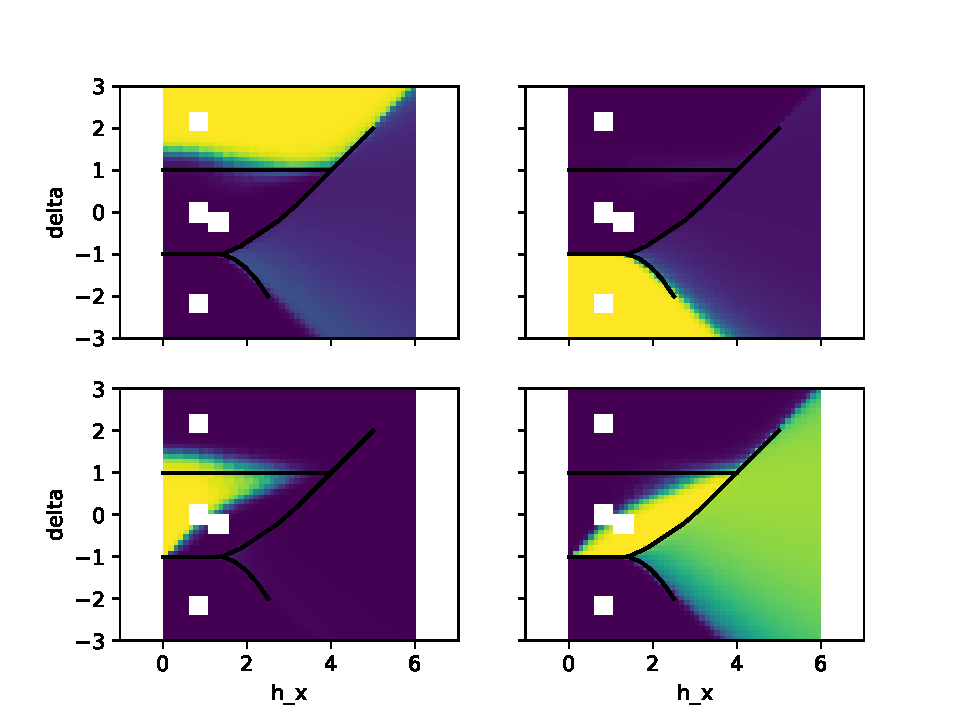
\includegraphics[width=\columnwidth]{3_6_Weak4PhaseDetection2D_134_20190119}
		
		\caption{Previous figure in different representation (same representation as in thesis)}
	\end{figure}

	We will now continue with the second question regarding robustness. Is it possible to detect an erroneous phase guess? Consider an initial guess as presented in figure \ref{fig:asymptotic:wrongguess}. The region of high $h_x$ is completely missing during training, but the region of low $\Delta$ and $h_x$ is labeled with 2 different labels. This forces the classifier to find differences in the correlation functions within region 3 and is able to find two continuous regions similar to training data in each of the patches. As these patches are moved, the inaccurately predicted decision boundary is very dynamic and behaves similar to the crossover boundary. This lack of robustness can be a method to detect and correct such a mistake of over-specifying phases during the initial guess. 
	
	As for the opposite case: The phase that did not contain any training data at all is clearly outlined in the gradient phase diagram in figure \ref{fig:asymptotic:wrongguess}. Within that phase, the classifier is not very confident for any of the classes and splits the confidence roughly as (0.2, 0.2, 0, 0.6) across the four class labels, almost constant over the entire region. The 60\% confidence neuron corresponds to the label of the training patch of highest $h_x$, the confidence of 0 corresponds to the training patch where $\Delta=0$.
	
	
	
	\section{Conclusion}
	We have recovered the two-dimensional phase diagram of the one-dimensional XXZ-Heisenberg model using both the confusion scheme and our newly-introduced asymptotic learning. The confusion scheme is completely unsupervised but does depend on a careful selection of the hyperparameters scan direction and window size while the asymptotic scheme requires an initial phase guess. The predicted boundaries of the confusion scheme even with the smallest window size possible for the given dataset are much broader than those of the asymptotic scheme. Additionally, the confusion scheme produces a much noisier phase diagram. It did not predict the crossover. When comparing run times, the confusion scheme is 2-3 orders of magnitude slower than the asymptotic scheme. However, multiple iterations of the confusion scheme for different training data selections may need to be run to detect crossovers or erroneous phase guesses.
	
	Apart from the required phase guess, the asymptotic method has the same prerequisites as the confusion scheme and can therefore also be applied to any system to map out the phase diagram. We are aware the active-contours variant of the confusion scheme as introduced by \cite{Liu2017}, and argue that our initial asymptotic phase guess is assumption is easier to fulfill and requires less prior knowledge about the topology of the phase boundaries.
	
	Especially for more complicated order parameters, the global approach of this method may become a helpful tool of pattern recognition in quantum systems.
	
	
	\bibliography{../mastercode/thesis/library}
	
	
\end{document}